% mnras_template.tex 
%
% LaTeX template for creating an MNRAS paper
%
% v3.0 released 14 May 2015
% (version numbers match those of mnras.cls)
%
% Copyright (C) Royal Astronomical Society 2015
% Authors:
% Keith T. Smith (Royal Astronomical Society)

% Change log
%
% v3.0 May 2015
%    Renamed to match the new package name
%    Version number matches mnras.cls
%    A few minor tweaks to wording
% v1.0 September 2013
%    Beta testing only - never publicly released
%    First version: a simple (ish) template for creating an MNRAS paper

%%%%%%%%%%%%%%%%%%%%%%%%%%%%%%%%%%%%%%%%%%%%%%%%%%
% Basic setup. Most papers should leave these options alone.
\documentclass[fleqn,usenatbib]{mnras}

% MNRAS is set in Times font. If you don't have this installed (most LaTeX
% installations will be fine) or prefer the old Computer Modern fonts, comment
% out the following line
\usepackage{newtxtext,newtxmath}
% Depending on your LaTeX fonts installation, you might get better results with one of these:
%\usepackage{mathptmx}
%\usepackage{txfonts}

% Use vector fonts, so it zooms properly in on-screen viewing software
% Don't change these lines unless you know what you are doing
\usepackage[T1]{fontenc}

% Allow "Thomas van Noord" and "Simon de Laguarde" and alike to be sorted by "N" and "L" etc. in the bibliography.
% Write the name in the bibliography as "\VAN{Noord}{Van}{van} Noord, Thomas"
\DeclareRobustCommand{\VAN}[3]{#2}
\let\VANthebibliography\thebibliography
\def\thebibliography{\DeclareRobustCommand{\VAN}[3]{##3}\VANthebibliography}


%%%%% AUTHORS - PLACE YOUR OWN PACKAGES HERE %%%%%

% Only include extra packages if you really need them. Common packages are:
\usepackage{graphicx}	% Including figure files
% \usepackage{amsmath}	% Advanced maths commands
% \usepackage{amssymb}	% Extra maths symbols (this seems to be already defined)
\usepackage{cuted}
\setlength{\stripsep}{0ex}

%%%%% AUTHORS - PLACE YOUR OWN COMMANDS HERE %%%%%

\newcommand{\todo}[1]{{\bf \color{red} #1}}
\newcommand{\notes}[1]{{\color{cyan} #1}}

\newcommand{\Gradus}{Gradus.jl}

\newcommand{\e}{\text{e}}
\renewcommand{\d}{\text{d}}
\newcommand{\utensor}[3]{#1^{#2}_{\phantom{#2}#3}}
\newcommand{\dtensor}[3]{#1_{#2}^{\phantom{#2}#3}}
\newcommand{\stensor}[3]{#1_{#2}^{#3}}
\newcommand{\deriv}[2]{\frac{\d #1}{\d #2}}
\newcommand{\pderiv}[2]{\frac{\partial #1}{\partial #2}}

\newcommand{\vel}[1]{v^{#1}}
\renewcommand{\vector}[1]{\mathbf{#1}}

%%%%%%%%%%%%%%%%%%% TITLE PAGE %%%%%%%%%%%%%%%%%%%

\title[Gradus.jl]{Gradus.jl: extensible and spacetime agnostic general relativistic ray-tracing for reverberation modelling through automatic differentiation}

% The list of authors, and the short list which is used in the headers.
% If you need two or more lines of authors, add an extra line using \newauthor
\author[F. J. E. Baker et al.]{
F. J. E. Baker,$^{1}$\thanks{E-mail: fergus.baker@bristol.ac.uk (FB)}
and A. J. Young$^{1}$
% Plus other contributing authors (tbc)
\\
% List of institutions
$^{1}$H. H. Wills Physics Laboratory, Tyndall Avenue, Bristol BS8 1TL, UK
}

% These dates will be filled out by the publisher
\date{Accepted XXX. Received YYY; in original form ZZZ}

% Enter the current year, for the copyright statements etc.
\pubyear{2023}

% Don't change these lines
\begin{document}
\label{firstpage}
\pagerange{\pageref{firstpage}--\pageref{lastpage}}
\maketitle

% Abstract of the paper
\begin{abstract}
	We introduce \Gradus, an open-source...
\end{abstract}

% Select between one and six entries from the list of approved keywords.
% Don't make up new ones.
\begin{keywords}
keyword1 -- keyword2 -- keyword3
\end{keywords}

%%%%%%%%%%%%%%%%%%%%%%%%%%%%%%%%%%%%%%%%%%%%%%%%%%

%%%%%%%%%%%%%%%%% BODY OF PAPER %%%%%%%%%%%%%%%%%%

%% INTRODUCTION
\section{Introduction}

\notes{
In the era of quantitative, precision observational tests of General Relativity in the strong field regime it is necessary to have a fast and flexible method to compute the observational properties of accreting black hole systems. We have developed an open-source integrator 
\Gradus\footnote{Open-source and available under MIT license at \url{https://github.com/astro-group-bristol/Gradus.jl}.} for this purpose. In the remainder of the paper we describe how the software works, comparing with previous work in the literature, and outlining the new capabilities of \Gradus.

% Maybe some history of the problem with key references
Transfer functions \citep{cunningham_effects_1975} % An example reference

Julia is a high-performance... with SciML and DifferentialEquations.jl, a state-of-the-art ecosystem and workhorse for solving differential equations. 
}


The trajectory of light in curved space may be determined by reformulating the Hamilton-Jacobi equations of motion as a first-order ordinary differential equation (ODE) system. 

A second-order ODE system may alternatively be formulated directly from the geodesic equation; a method which is pedagogically simpler, but computationally more expensive than the first-order system, as either the full metric connection or derivatives of the metric must be explicitly implemented, else approximated at cost during runtime. With advancements in automatic differentiation, derivatives are cheap to compute, and consequently the second-order approach is tractable and both a parsimonious and spacetime agnostic method for computing geodesics.

%% NUMERICAL METHODS
\section{Numerical methods}

For simplicity, we will here focus on static, axisymmetric spacetimes in the Boyer-Lindquist coordinates. Such a spacetime has a metric of the form 
\begin{equation}
\label{eq:static_axisymmetric_metric}
    g_{\mu\nu} 
    = g_{tt} \d t^2 
    + g_{rr} \d r^2 
    + g_{\theta\theta} \d \theta^2 
    + g_{\phi\phi} \d \phi^2 
    + 2g_{t\phi} \d t \d \phi.
\end{equation}
We adopt $(-, +, +, +)$ signature and standard units $c = G = 1$. Greek indices ($\mu, \nu$) will be used to denote the four spacetime components, and Latin indices ($i, j$) for the three spatial components. We write partial derivatives with respect to the coordinates $x^\mu$ as $\partial_\mu := \partial / \partial x^\mu$.


%% SECTION: GEODESIC INTEGRATION
\subsection{Geodesic integration}

The geodesic equation with coordinates $x^\mu$ is
\begin{equation}
\label{eq:geodesic_equation}
    \frac{\d^2 x^\mu}{\d \lambda^2}
    + \utensor{\Gamma}{\mu}{\nu\sigma}
    \vel{\nu}
    \vel{\sigma}
    = a^\mu,
\end{equation}
where $\lambda$ is the affine parameter, $v^\mu = \d x^\mu / \d \lambda$ is the four-velocity, and $a^\mu$ is some external acceleration. The effects of curvature on the trajectory are encoded in the Christoffel connections, 
\begin{equation}
\label{eq:christoffel}
    \utensor{\Gamma}{\mu}{\nu\sigma}
    := \frac{1}{2} g^{\mu\rho} 
    \left(
        \partial_{\nu}g_{\rho \sigma}
        + \partial_{\sigma}g_{\rho \nu}
        - \partial_{\rho}g_{\sigma \nu}
    \right),
\end{equation}
determined solely by metric and derivatives thereof. For a given metric, the geodesic equation is a set of four coupled second order differential equations that may be solved for a choice of initial $x^\mu$ and $\vel{\mu}$. The convention is to choose an initial position with $x^t = 0$, whereas the velocity vector is additionally constrained by the invariance
\begin{equation}
\label{eq:velocity_constraint}
    g_{\sigma\nu} \vel{\sigma} \vel{\nu} = \mu^2,
\end{equation}
where $\mu$ is the invariant mass. This invariance gives rise to three solution classes depending on the sign of $\mu^2$, namely $\mu^2 = 0$ corresponding to null-, $\mu^2 > 0$ to time-, and $\mu^2 < 0$ to space-like geodesics. Null geodesics are the trajectories of photons, time-like geodesics are the trajectories of massive particles, and space-like geodesics are the trajectories of exotic particles, such as tachyons. Specifying the three-vector $\vel{i}$ determines $\vel{t}$ by Eq. \eqref{eq:velocity_constraint}, rearranged as
\begin{equation}
\vel{t}  = \frac{-g_{t\phi} \vel{\phi} \pm
    \sqrt{-g_{ij} \vel{i} \vel{j} - \mu^2}
}{g_{tt}}.
\end{equation}
The choice of positive or negative root corresponds to the direction of time, wherein lies the ray-tracing \textit{trick}: a time-reversal symmetry in the metric allows us to trace from an observer back to the point of origin, and then \textit{reverse} time in order to calculate quantities as seen by the observer. \todo{explain better}

The integration of the ODE system is performed numerically with an appropriate choice of algorithm. We favour the adaptive Tsitouras Runge-Kutta 5/4 \citep{tsitouras_rungekutta_2011}. This integrator is shown to be fast and robust, also providing free fourth-order interpolants of the resulting geodesics. The interpolants can be particularly useful if additional quantities need to be re-traced along a geodesic, or for accurately finding points of intersections.

Derivatives of the metric needed in Eq. \eqref{eq:christoffel} may be efficiently computed with AD. This brings versatility and ease, as new spacetimes need only to define the metric for the geodesic system to be computable, and AD ensures the derivatives are free of the pathologies of other e.g. stenciling methods used to compute derivatives. If the class of spacetime exhibits additional symmetries, these can be exploited to reduce computation further: metrics of the form \eqref{eq:static_axisymmetric_metric} can exploit $\partial_t g_{\mu\nu} = \partial{\phi} g_{\mu\nu} = 0$ and avoid calculating two columns of the Jacobian entirely.

Sparsity is often symbolically inferable under simple operations. We use compile time Julia \texttt{@generated} functions, along with Symbolics.jl, to attempt to infer which terms in the Jacobian and Christoffel symbols can be avoided (if any), to generate optimal evaluation for a given class of metric. 
%This was benchmarked against other packages that perform the sparsity detection generically, such as FastDifferentiation.jl, and find similar performance.


\subsection{Observers and emitters}

\begin{figure}
    \centering
    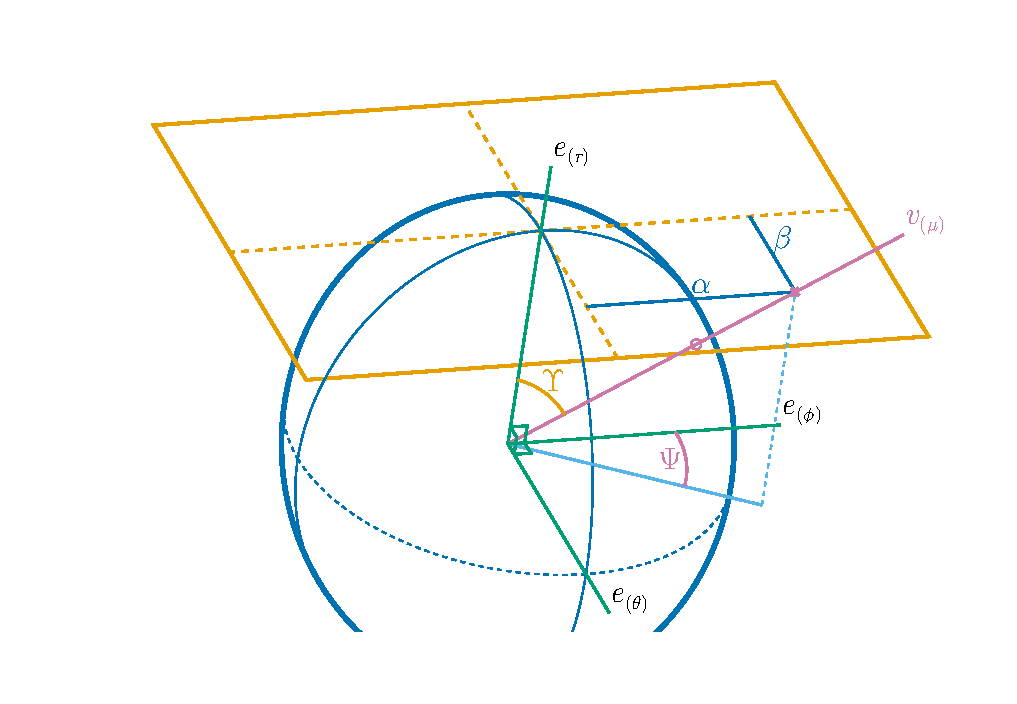
\includegraphics[width=0.99\linewidth]{figures/skycoords.pdf}
    \caption{Geometry of the local sky for an observer or emitter. The image plane is perpendicular to the $e_{(r)}$ axis, which for an observer points towards the global origin and therefore the central singularity. The momenta $v_{(\phi)}$ and $v_{(\theta)}$ are used to calculate the impact parameters on the image plane, $\alpha$ and $\beta$ respectively. For emitters, the angles $(\Upsilon, \Psi)$ are used to parameterize points on the local sky, that may be decomposed onto the basis $e_{(i)}$ to find $v_{(\mu)}$.}
    \label{fig:observer-coordinates}
\end{figure}

To determine interpretable initial velocities it is useful to consider the coordinates local to the observer or emitter at coordinates $x^\mu$. For observers one usually an image plane onto which a projection of geodesics is rendered, with geometry as in Fig. \ref{fig:observer-coordinates}. Following \cite{cunningham_optical_1973}, one may then define a set of impact parameters from components of the local momenta
\begin{align}
    \alpha &:=  x^r \frac{v_{(\phi)}}{v_{(r)}}, \\
    \beta &:= x^r \frac{v_{(\theta)}}{v_{(r)}},
\end{align}
using indices in parentheses to denote the vector components in the local frame. The choice of subscript ($r, \theta, \phi$) is to anticipate an identification between local and global bases, and to provide some intuition for the local frame.

Along with the invariance of four-momenta (c.f. Eq. \eqref{eq:velocity_constraint}), one may obtain a curve of solutions for the local momenta
\begin{align}
    \frac{v_{(r)}}{v_{(t)}} &= -\left( \sqrt{1 + \left(\frac{\alpha}{x^r}\right)^2 + \left(\frac{\beta}{x^r}\right)^2} \right)^{-1} = \mathscr{R}, \\
    \frac{v_{(\theta)}}{v_{(t)}} &= \mathscr{R} \frac{\beta}{x^r}, \\
    \frac{v_{(\phi)}}{v_{(t)}} &= \mathscr{R} \frac{\alpha}{x^r}.
\end{align}

For emitters, one determines these momenta from an initial velocity tangent vector pointing along a direction on the local sky, parameterized by local angles $(\Upsilon, \Psi)$, as in Figure \ref{fig:observer-coordinates}. Using simple geometry and projecting the local angles onto a Cartesian coordinate system gives momenta
\begin{equation}
    \frac{v_{(i)}}{v_{(t)}} = \frac{1}{v_{(t)}}
    \left[\pderiv{(x, y, z)}{(r, \theta, \phi)}\right]
    \left(
    \begin{matrix}
        \sin \Upsilon \cos \Psi \\
        \sin \Upsilon \sin \Psi \\
        \cos \Upsilon \\
    \end{matrix}
    \right),
\end{equation}
where the partial derivative term denotes the cartesian to spherical coordinate Jacobian. The component $v_{(t)}$ is the negative of the energy measured in the local frame, and is conventionally set to $-v_{(t)} = E = 1$ without loss of generality. 

For both observers and emitters, we must identify a local frame, where the natural choice is the locally non-rotating frame (LNRF) \citep{bardeen_rotating_1972} \todo{check citation + explain significance}. The transformation from local to global coordinates is
\begin{equation}
    v_\mu = \e^{(\nu)}_{\phantom{(\nu)}\mu}\  v_{(\nu)}
\end{equation}
where the basis vectors $\e^{(\nu)}_{\phantom{(\nu)}\mu}$ (or tetrad) are found using the theorem of Gram-Schmidt (\citealp{schmidt_uber_1989}, Appendix \ref{appendix:gram-schmidt}). The formalism may be extended for an observer or emitter in motion, where their velocity modifies the mapping by a local Lorenz transformation, $\Lambda^{(\kappa)}_{\phantom{(\kappa)}(\nu)}$, as 
\begin{equation}
    v_\mu = \e^{(\nu)}_{\phantom{(\nu)}\mu}\  \Lambda^{(\kappa)}_{\phantom{(a)}(\nu)} v_{(\kappa)}.
\end{equation}
However, this Lorenz transformation may be absorbed into the tetrad with careful construction, using the velocity of the observer or emitter as $\utensor{\e}{(t)}{\mu}$.

Expressions for the impact parameters from the constant of motion in \cite{cunningham_optical_1973} always assume that the observer is situated in asymptotically flat space, whereas our calculations are specific to the location of the observer. This should be taken into account when comparing trajectories between codes and methods.

\subsection{Special orbits and horizons}
\label{sec:special-orbits}

For many disc models, accreting matter is considered to follow Keplerian circular orbits in the equatorial plane $(x^\theta = \pi/2)$ of the central singularity \citep{shakura_black_1973}. These Keplerian circular orbits are stationary points of the Hamiltonian and constrained by $v^r = v^\theta = 0$. For static, axis-symmetric spacetimes, these orbits may be studied analytically (e.g. \citealp{johannsen_regular_2013}, with a variation of their derivation and extension for $a^\mu \neq 0$ in Appendix \ref{appendix:circular-orbits}).

In general relativity, circular orbits are classified as either stable or unstable \citep{wilkins_bound_1972,bardeen_rotating_1972}. There exists an innermost stable circular orbit (ISCO) radius, below which orbits are energetically hyperbolic: small perturbations will send the test particle escaping to infinity or spiralling into the central singularity.  Stability of an orbit depends on the sign of $\d E / \d x^r$, with $>0$ corresponding to energetically stable configurations, such that the ISCO is the critical point at which 
\begin{equation}
    \label{eq:isco-definition}
    0 = \left. \frac{\d E}{\d x^r} \right\rvert_{x^r := r_\text{ISCO}}.
\end{equation}
Stable circular orbits are only possible for radii $x^r \geq r_\text{ISCO}$. Within the ISCO is the so-called \textit{plunging region} where $v^r \neq 0$. 


Orbits may also be determined purely from the integration of geodesics, by mandating a stability measure and optimizing the initial velocity vector until some heuristic measure is a minimum. For example, let $\mathscr{M}$ measure the eccentricity of an orbit in the equatorial plane. For a given radius $x^r$, the velocity corresponding to a circular orbit is $v^\mu = v^t \partial_t + v^\phi \partial_\phi $. With \eqref{eq:velocity_constraint}, the circular orbit velocity may be found through
\begin{equation}
    \underset{v^\phi}{\arg \min}\ \ \mathscr{M}(x^r, v^\phi),
\end{equation}
using a numerical optimizer. We use the Nelder-Mead simplex method as our preferred optimization algorithm for exploring the $v^\phi$ parameter space \citep{nelder_simplex_1965}. Due to only integrating finite windings of the orbit, this approach may find both unstable and stable orbits. These may be distinguished by inspecting $E$ as a function of $x^r$, or similarly $E$ as a function of $L_z$ \citep{hackmann_charged_2013}, see Figure \ref{fig:e-lz-cusp}. The $r_\text{ISCO}$ is found by determining \eqref{eq:isco-definition} numerically, or by finding $x^r$ corresponding to the \textit{cusp} of the $E$ against $L_z$ plot.

\begin{figure}
    \centering
    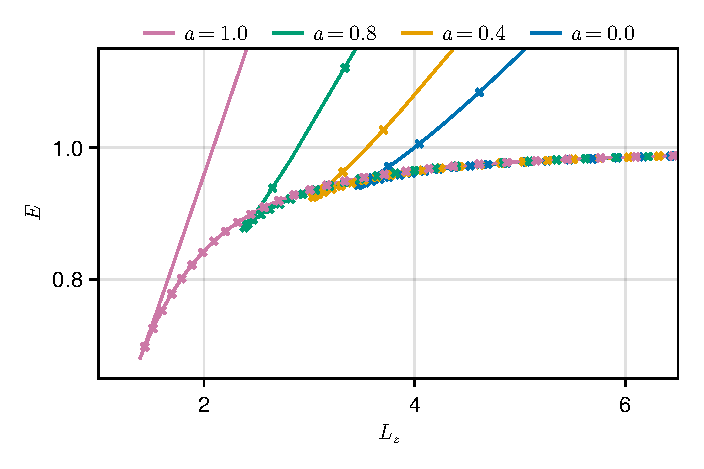
\includegraphics[width=0.95\linewidth]{figures/circular-orbits.E-Lz.pdf}
    \caption{\todo{TODO, also show the points we calculate using the numeric orbit finder}}
    \label{fig:e-lz-cusp}
\end{figure}

The velocity of plunging region orbits may be numerically calculated by ``dropping'' a test particle from $r_\text{ISCO} -  \delta x^r$, and tracing for a large interval of proper time. The components of $v^\mu$ may then be interpolated over $x^r$ to approximate analytic solutions. Figure \ref{fig:circular-orbit-error} illustrates the accuracy of our numerical method for determining orbits.

The heuristic minimization is also used for other objective functions, such as for pinpointing geodesics that intersect a chosen point in the spacetime ($\mathscr{M}$ measures closest approach), or exhibit some specific desired features (e.g. $\mathscr{M}$ measures periodicity).

\todo{solving for radii / horizons}
We use root solvers from Roots.jl \citep{}. The default we use is their ``Order 0'' solver, a hybrid method that refines from secant to bracketing methods when possible.

\notes{
How we find circular orbits, how we find ISCO, photon radius, event horizon
}


\subsection{Charts and horizons}

A chart is used to terminate geodesic integration to avoid continuing computation when the fate of a given geodesic is determined. In practical terms, the chart is defined by a set of boundaries, and used to classify the outcome of an integration. As a motivating example, consider a chart with an inner and outer boundary: the inner boundary is a coordinate singularity of the metric, $r_s$ (i.e. an event horizon), whereas the outer boundary is treated as the \textit{effective infinity}, $r_\infty$. Geodesics at the inner boundary are classified as lost behind the coordinate singularity, whereas those that reach the outer boundary are considered to escape to infinity with no further deviation to their trajectory. Additional boundaries of the chart may be used to represent accretion geometry: by terminating the integration when the geodesic crosses such a boundary, we consider the geodesic to have intersected the surface of the accretion disc. 

The event horizon radius, $r_s$, used as the default inner boundary, may be calculated for a metric of the form \eqref{eq:static_axisymmetric_metric} by solving
\begin{equation}
    \label{eq:event_horizon}
    0 = \left. \frac{1}{g_{rr}} \right\rvert_{x^r = r_s}.
\end{equation}
For axisymmetric metrics, $g_{rr}$ may be a function of both $x^r$ and $x^\theta$, in which case the inner boundary of the chart is a function of the poloidal coordinate. If no analytic function for $r_s$ is known, it may be numerically approximated using root solving methods.

In practice, close to the inner radius the adaptive time step of an ODE integrator tends to shrink dramatically due to near-singular derivatives, causing the integration to slow to almost a standstill. This may be avoided by scaling the inner horizon with the choice of constant $\mathcal{K} > 0$, such that $\tilde{r}_s = (1 + \mathcal{K}) r_s$, terminating the integration early when $x^r \leq \tilde{r}_s$. This constant may be adjusted depending on how vital it is for a geodesic to be able to glance the event horizon. We have chosen $\mathcal{K} = 10^{-2}$ by default, as it dramatically improves integration time without impacting the majority of simulations. 

Chart intersection is found using either an interpolating root-solver with \texttt{ContinuousCallback} or a per-point test with \texttt{DiscreteCallback} from DifferentialEquations.jl \citep{}.


\subsection{Computing observables}

We consider \textit{observables} to be any physical quantity calculated from a simulation that is evaluated using some or all of the points along a geodesic. Often only the start and end point of a geodesic are required to calculate some physical quantity, and under such circumstances it is computational beneficial to avoid allocating space for the full solutions.

A frequently required quantity is the redshift along a geodesic, due to both the Doppler and gravitational redshift. This is compactly written as the ratio of energies between the start and end point connected by the geodesic,
\begin{equation}
\label{eq:redshift}
g := \frac{E_\text{end}}{E_\text{start}} = \frac{\left. v_\mu u^\mu \right\rvert_\text{end}}{\left. v_\mu u^\mu \right\rvert_{\text{start}}},
\end{equation}
where $v_\mu$ are the photon momenta, and $u^\mu$ the velocity of the emitting (start) and observing (end) media respectively.

Observables that require multiple points along the geodesic to be determined may either be calculated coincidentally with the geodesic equation, or subsequently re-traced along the ray. Such quantities include polarization / parallel transport or radiative transfer / optical depth. Calculating the quantities simultaneously has the benefit that the error tolerance in the step size estimation of the integrator is sensitive to changes in the observable. The benefit of the latter is that for a given set of metric parameters and observer inclination, the geodesics trajectories are unchanged, allowing the observable to be more efficiently recalculated with new parameters.

\subsection{Covariant radiative transfer}

The intensity of a given geodesic is an observable that can be either calculated coincident with the geodesic trajectory, or retraced once the trajectory is determined.

The covariant formulation of the radiative transfer equation calculates the emissions and extinction in aframe co-moving with the geodesic \citep{fuerst_radiation_2004,younsi_general_2012}. The generalized form of the differential equation with respect to the affine parameter $\lambda$ is
\begin{equation}
    \label{eq:covariant-radiative-transfer}
    \frac{\d \mathcal{I}}{\d \lambda} = \left. \frac{\d s}{\d \lambda} \right\rvert_\lambda \left( -\alpha_\nu \mathcal{I} + \frac{j_\nu}{\nu^3} \right),
\end{equation}
where $\mathcal{I}$ is the invariant intensity, $s$ is the proper length traversed by the geodesic, and $\alpha_\nu$ and $j_\nu$ are the frequency $\nu$ dependent absorption and emissivity coefficients respectively, as measured in the local frame. The frequency $\nu$ is related to the observed frequency via the redshift
\begin{equation}
    g = \frac{\nu_\text{obs}}{\nu},
\end{equation}
In general, both coefficients $\alpha_nu$ and $j_\nu$ are also functions of the position $x^\mu$. 

The $\d s / \d \lambda$ derivative term is calculated by projecting the geodesic momentum $v_\mu$ onto the velocity $u^\mu$ of the medium, using the projection tensor
\begin{equation}
    \mathrm{P}^{\mu\nu} := g^{\mu\nu} + u^\mu u^\nu.
\end{equation}
The path length derivative is 
\begin{align}
    \left. \frac{\d s}{\d \lambda} \right\rvert_\lambda
    &= - \left. \left\lVert \mathrm{P}^{\mu\nu} v_\mu\right\rVert\, \right\rvert_\lambda,\\
    &= - \left. \sqrt{v_\mu v^\mu + \left(v_\mu u^\mu\right)^2 \left(2 + u^\mu u_\mu\right)} \, \right\rvert_\lambda,
\end{align}
such that for the particular case of null geodesics through a time-like medium
\begin{equation}
    \left. \frac{\d s}{\d \lambda} \right\rvert_\lambda = - \left. v_\mu u^\mu \right\rvert_\lambda.
\end{equation}

The covariant intensity $\mathcal{I}$ is related to the observed intensity $I_\nu = \mathcal{I} \nu^3$, derived using Liouville's theorem. The intensity is therefore calculated by selecting $\nu_\text{obs} = E$ at the observer, and integrating \eqref{eq:covariant-radiative-transfer} along a given geodesic. 


\subsection{Emissivity profiles}

The emissivity of a disc is defined as the flux emitted from the disc, such that the emissivity profile is the flux as a function of the disc coordinates \citep{wilkins_understanding_2012}. For reflection, the flux emitted is proportional to the flux received from the illuminating corona \citep{laor_line_1991}. As axis-symmetry of the accretion disc emissivity profile is usually manifest, the emissivity profile is a function of the radial coordinate on the accretion disc and given by
\begin{equation}
    \varepsilon (r, \d r) = \frac{\mathcal{N}(r, \d r)}{\gamma A(r, \d r)} I(g),
\end{equation}
where $\mathcal{N}$ is the photon count in an annulus $r + \d r$, $I$ is the intensity of the illuminating flux as a function of redshift $g$, $A$ is the relativistically corrected (proper) area of the annulus, and $\gamma$ is the Lorentz factor account for contraction of the annulus due to the velocity of the disc.

The intensity function for the illuminating corona is usually assumed to be a powerlaw $I(g) = g^{-\Gamma}$ with varying photon index $\Gamma$ \citep{gonzalez_probing_2017}.

An alternative method for calculating the flux from point sources is detailed in \cite{dauser_irradiation_2013}, where the axis-symmetry is further exploited. This method determines the radii of the annuli by tracing photons that are emitted at equally spaced angles $\Delta \theta$ in the source frame, and using the radial coordinate of geodesics where they intersect the disc $\Delta r$ as a proxy for the reciprocal number density. Since in three spatial dimensions, the poloidal coordinate must be distributed as a $\sin \theta$ distribution for isotropic emission, $\varepsilon$ is weighted similarly\footnote{Instead of equally spaced $\theta$, one may instead sample $\theta \sim \cos (1 - 2 \mathcal{U})$, where $\mathcal{U}$ is a uniform distribution $\mathcal{U}(0,1)$. In this case, there is no $\sin \theta$ weight in $\varepsilon$. This result may be shown using the inverse-CDF or Smirnov transform method.}
\begin{equation}
    \varepsilon(r, \Delta r) = \frac{\sin \theta}{\gamma A(r, \Delta r)} I(g).
\end{equation}
The differences between these two methods is shown in Figure \ref{fig:coronal-tracing}. It should be noted that the latter method converges faster than the (Monte-Carlo) sampling of $\mathcal{N}$, and captures the behaviour at small $r$ close to the ISCO faithfully. However, since this method is specialized for point sources, extended corona require an approximate rebinning algorithm to reconstruct the emissivity profile taking into account the overlap between the annuli determined from different source points.

\begin{figure}
    \centering
    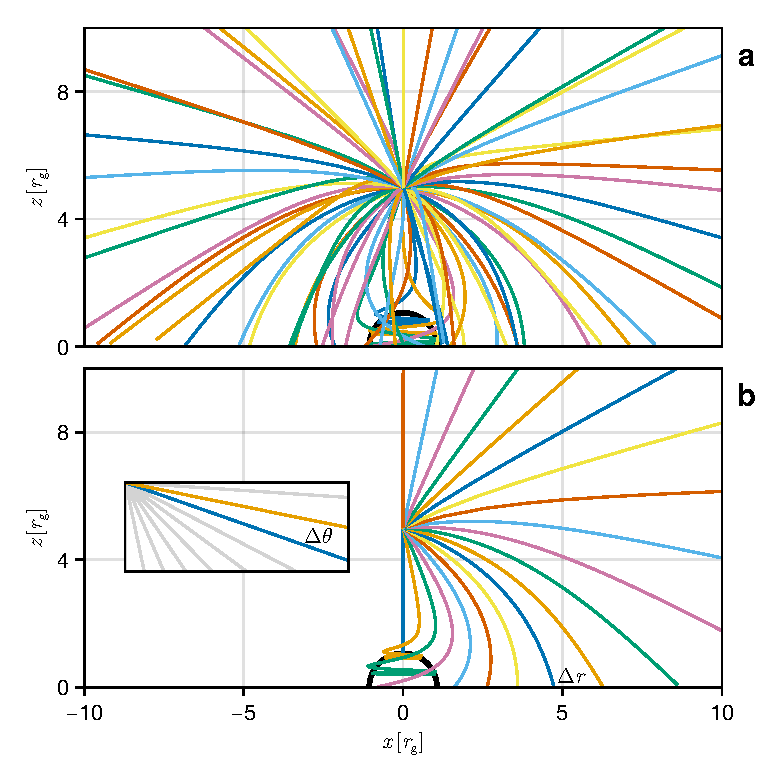
\includegraphics[width=0.95\linewidth]{figures/emissivity.coronal-traces.pdf}
    \caption{\todo{caption}}
    \label{fig:coronal-tracing}
\end{figure}

When axis-symmetry does not apply, we have developed a method for calculating the emissivity field as a function of $(r, \phi)$ on the disc. Here the point of intersection on the disc become the generators of a Delauney tesselation, such that the Voronoi (proper) area may be used as a proxy for $\mathcal{N} / A$ (see Appendix \ref{appendix:voronoi}) in the limit of high sample count.

\subsection{Transfer functions}

A particular observable that is frequently calculated with GRRT is the flux coming from a particular model of an accreting black hole. The infinitesimal flux is
\begin{equation}
\d F(E, t) = I\left(E, t\right)\, \d \Omega,
\end{equation}
for observed energy $E$, time $t$, intensity $I$ and solid angle $\d \Omega$ on the observer's sky.

Using Liouville's theorem -- that the number density of photons in phase space is conserved -- the observed and emitted intensities are related by
\begin{equation}
    I\left( E, t \right) = g^3 I_\text{em}\left(E_\text{em}, t_\text{em}\right).
\end{equation}
\todo{is this $t_\text{em}$ or just $t$??}
Integrating over $\d \Omega$ is equivalent to integrating over the image plane $\d \alpha \d \beta$, which in practical terms is binning the geodesic in each pixel by $E$ and $t$. In this formulation, for any change in $I_\text{em}$, the geodesic calculation would have to be recomputed, or a large table of values related to each geodesic stored, to finite precision. The sampling over the image plane similarly plays an important role, especially in increasing efficiency, since most of the variation in $I_\text{em}$ is sourced close to the ISCO, which can be under-resolved on coarse image planes. This may lead to oversampling regions of low or zero variation further out on the disc.

\begin{figure}
    \centering
    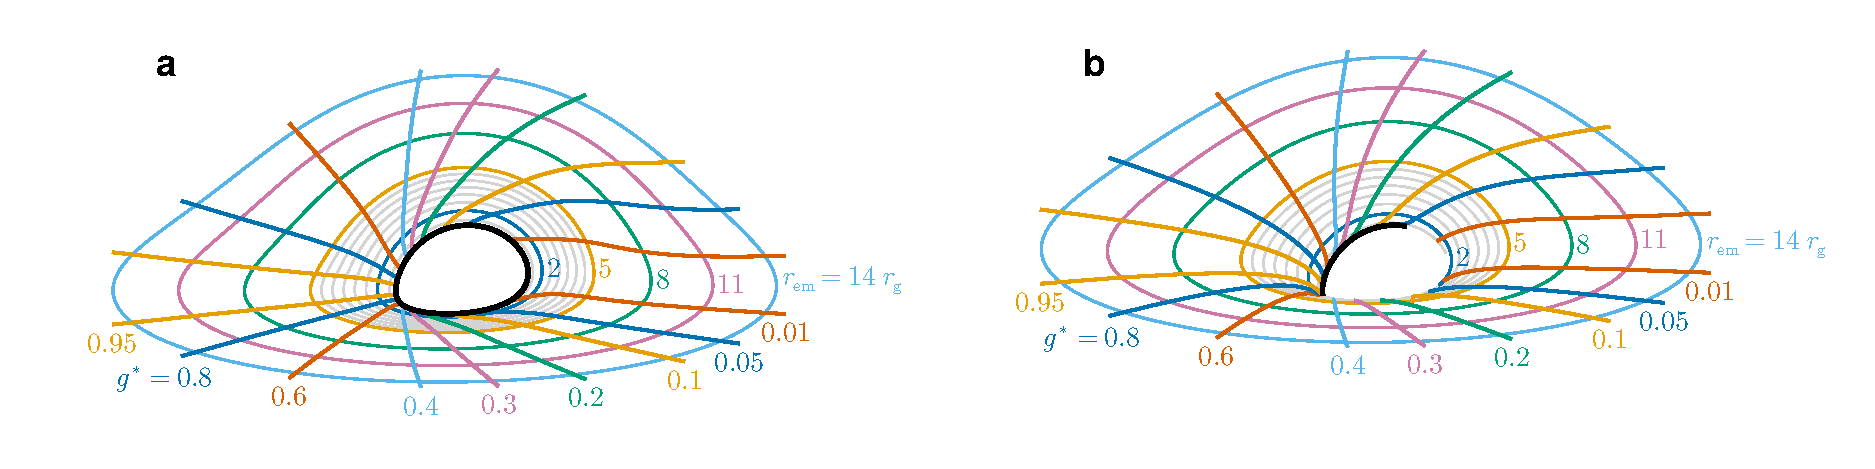
\includegraphics[width=0.95\linewidth]{figures/transfer-function.parameterization.pdf}
    \caption{\todo{caption}}
    \label{fig:transfer-parameterisation}
\end{figure}

To elide this problems, and to be able to succinctly cache geodesic computation, the relativistic effects are often encoded in so-called \emph{transfer functions}, first introduced in \cite{cunningham_effects_1975},
\begin{equation}
    f:=\frac{g}{\pi r_\text{em}} \sqrt{g^\ast(1 - g^\ast)} \jacobian{(\alpha, \beta)}{(r_\text{em}, g^\ast)},
\end{equation}
where $r_\text{em}$ is the emission radius on the disc, and
\begin{equation}
    g^\ast := \frac{g - g_\text{min}}{g_\text{max} - g_\text{min}} \in [0, 1],
\end{equation}
is a rescaled dimensionless redshift parameter, and the extremal $g$ is calculated over a given $r_\text{em}$. This $g^\ast$ parameterization is double-valued everywhere except at $g^\ast = 0$ and $g^\ast = 1$, illustrated in Figure \ref{fig:transfer-parameterisation}. The transfer functions $f$ are then ostensibly a change-of-variable Jacobian, re-parameterizing the projected image of the disc from $(\alpha, \beta)$ to $(r_\text{em}, g^\ast)$. The additional elliptical envelope in $g$ supresses the singular values of the Jacobian as $g^\ast$ becomes $0$ or $1$, permitting numerical integration of the transfer function with fewer issues. To avoid the double-valued degeneracy when integrating, the transfer functions are in practice split into an ``upper'' and ``lower'' branch, between extremal $g^\ast$, shown in Figure \ref{fig:transfer-functions} with the light-travel time of the geodesic similarly constructed. Furthermore, with the disc projection given in terms of quantities on the disc allows physical emission models to be specified in the local emitting frame.

Our method for calculating the transfer functions is a variation on the algorithms detailed by other authors (\citealp{speith_photon_1995,bambi_testing_2017}, improved in \citealp{abdikamalov_public_2019}). The procedure is as follows: first, we find the impact parameters that map to a ring of radius $r_\text{em}$ on the accretion disc. In the case of simple axis-symmetric discs, the projection of a ring will be the boundary of a star-convex set on the image plane, and therefore a polar curve $\mathcal{R}(\vartheta)$, with $\alpha = \mathcal{R}(\vartheta) \cos(\vartheta)$ and $\beta = \mathcal{R}(\vartheta) \sin(\vartheta)$. For a given $\vartheta$, the offset on the image plane $\mathcal{R}$ is found by root-finding the difference between $r_\text{em}$ and the projected endpoint of the geodesic on the disc $r = x^r (\mathcal{R}) \sin x^\theta(\mathcal{R})$, using the same alternating root finder as in Section \ref{sec:special-orbits}.

For a given $r_\text{em}$, the extremal $g$ are found by using the Golden-Section bracketing method to extremize $g(\vartheta)$, with the assumption that extremal $g$ approximately coincide with extremal $\alpha$. Informed by this, we use $\vartheta \in [ -\pi/2, 3\pi/4 )$ to ensure the maxima and minima are not at the boundaries of the domain. \todo{want to say more about how difficult finding extremal $g$ is / how important getting good estimates is??}

The Jacobian is more conveniently calculated as
\begin{equation}
    \left\lvert 
    \pderiv{(\alpha, \beta)}{(r_\text{em}, g^\ast)} 
    \right\rvert
    =
    \left\lvert
    \pderiv{r_\text{em}}{\alpha}\pderiv{g^\ast}{\beta}
    -
    \pderiv{r_\text{em}}{\beta}\pderiv{g^\ast}{\alpha}
    \right\rvert^{-1},
\end{equation}
where the derivatives have previously been determined using a stenciling approach to determine the Jacobian term, or even just a fixed $\delta \alpha$ and $\delta \beta$. Unless the algorithm can adapt extremely well, these approaches may introduce singular values or risk large numerical error at extremal $g$. We instead use AD to directly calculate the inverse of the Jacobian, which has the additional benefit that it only requires the evaluation of a single geodesic to compute, as is thus substantially faster.


\begin{figure}
    \centering
    \caption{\todo{caption}}
    \label{fig:transfer-functions}
\end{figure}

\subsection{Integrating transfer functions}

Integrating $\d F(E)$ to calculate line-profiles is described in detail in \cite{dauser_broad_2010}, including the Green's function formalism that adds additional flexibility in the definition of $I_\text{em}$. We extend the transfer function integration to include the geodesic coordinate time, integrating $f$ as

% \begin{strip}
% \rule[-1ex]{\columnwidth}{0.7pt}\rule[-1ex]{0.7pt}{1.5ex}
% \vbox{\vspace{2em}}
\begin{align}
    \label{eq:transfer-integration}
    F(E, t) &=
    \pi
    \int_0^\infty \d t^\prime \delta(t - t^\prime)
    \int_{r_\text{in}}^{r_\text{out}} \d r_\text{em}\,r_\text{em} \nonumber \\
    &\ \int_0^1 \d g^\ast\, \delta(E - gE_\text{line})\, g^2 I_\text{em}\left(\frac{E}{g}, t^\prime\right) \frac{f(r_\text{em}, g^\ast)}{\sqrt{g^\ast (1 - g^\ast)}},
\end{align}
% \vbox{\vspace{2em}}
% \hfill\rule[1ex]{0.7pt}{1.5ex}\rule[2.3ex]{\columnwidth}{0.7pt}
% \end{strip}
\noindent and $g = g( r_\text{em}, g^\ast, t')$ implicitly. The integrand remains in practice singular at $g^\ast \rightarrow (0, 1)$, and therefore the integration is performed over $g^\ast \in [h, 1 - h]$. Outside of this domain, the limits of the integrand can be taken to approximate the edges of the bin, as in \cite{dauser_broad_2010},
\begin{equation}
   F_\text{edge}(E,t) \propto 2\left( \sqrt{E_\text{max}} - \sqrt{E_\text{min}} \right).
\end{equation}
The constant of proportionality is determined from evaluating the integrand at $h$ or $1 - h$ respectively.

We use $h = 2 \times 10^{-8}$, and evaluate the integral over $\d g^\ast$ using a 7$^\text{th}$ order Gauss-Kronrod quadrature scheme, which avoids evaluating the integral directly at $h$ and $1 - h$ \citep{}. Finer grids for $r_\text{em}$ and $g^\ast$ are constructed to help with stability, and rebinned into the desired grid. 

The method for numerically integrating the transfer functions is as follows: the limits of the integral are chosen $(r_\text{in}, r_\text{out})$, and limits of the output space similarly $(E_\text{min}, E_\text{max})$, $(t_\text{min}, t_\text{max})$. Any evaluation of \eqref{eq:transfer-integration} that is outside of the energy and time limits is ignored. To ensure the approximate methods remain accurate, a fine grid in $r$ and $g$ is constructed\footnote{The grid in $r$ should be irregularly spaced, e.g. $\sim 1 / r$, whereas the grid in $g$ should be linear.}. The integration over $\d r_\text{em}$ is performed using a trapezoidal interpolation, which is sufficient in both accuracy and performance with the finer bins. Since the integration over $\d t$ has the selection effect of binning, we assign the flux $F(E)$ into time bin $t$ by considering $t$ over the width of $g^\ast$ on the fine grid. In full:
\begin{enumerate}
    \item Interpolate the values of the transfer function, $f$, $t$, and $g_\text{min}$, and $g_\text{max}$, for the current radius $r_i$.
    \item Calculate the trapezoidal integration weight for the radial coordinate, in effect $\omega_i = \Delta r_i r_i \varepsilon(r_i)$.
    \item For each bin in the fine $g$ grid, integrate $f$ over this bin. Record $t_\text{min} = t(g_\text{min})$ and $t_\text{max} = t(g_\text{max})$.
    \item Add $\omega_i F(E, t)$ to the bin corresponding to $E = gE_\text{line}$, and $t$. If either $\Delta E$ or $\Delta t$ straddles an output bin, the flux must be weighted appropriately and divided into those bins. 
\end{enumerate}

By formulating the integration with the time component, we can use the same transfer function table to compute both line-profiles and reverberation lags efficiently, with arbitrary intensity functions $I_\text{em}$. We note that extensions to $I_\text{em}$ that require, for example, the photon emission angle on the disc, are trivial to include.



%% DESCRIPTION OF THE CODE
\section{Description of the code}

\Gradus is implemented in the Julia programming language \citep{Bezanson_Julia_A_fresh_2017}. The code is available through popular package managers for a wide variety of languages, including Python via \texttt{pip}.

\Gradus aims to have a single expressive high-level API for a variety of GRRT problems, with sensible defaults and optional fine-grained control. The code is accompanied by rendered documentation\footnote{\url{https://astro-group-bristol.github.io/Gradus.jl/}}, with short tutorials and examples designed to provide a feature-rich overview whilst simultaneously demonstrating how to construct custom simulations and how to integrate \Gradus in a user's model. We encourage readers who are interesting in learning up-to-date information and method in our codes to consult the documentation over this paper. 

The documentation strives to be the most accurate description of the code as it is maintained, detailing algorithm specific choices and implementations, and is built as part of our continuous deployment (CD). The source code is written to be read by contributors and users alike to invite extension, and to be explicit about our methods, their benefits, and limitations.

In our discussion of the numerical methods, we note the current default ODE integration algorithm is Tsitouras Runge-Kutta 5/4. \Gradus vendors many additional ODE solvers and numerical algorithms from the Julia SciML ecosystem, with both adaptive and fixed time steps.

\Gradus maintains a catalogue of predefined metrics, including the Kerr spacetime, Morris-Thorne wormhole, Johannsen-Psaltis metric, the Einstein-Maxwell Dilaton-Axion metric \todo{citations for these}. The Kerr-Newman metric is also implemented, complete with the ability to specify the electromagnetic potential vector, from which external accelerations $a^\mu$ in \eqref{eq:geodesic_equation} are calculated. Furthermore, \Gradus allows for 1st order specification of the geodesic ODE system, where such a system is known. This is already implemented for the Kerr spacetime, and used primarily as a self-consistency check with the second-order implementation.

The AD in our code is from the ForwardDiff.jl package \citep{RevelsLubinPapamarkou2016}, and may be used when calculating any quantity or observable to simultaneously determine gradients.

\subsection{Parallelism and ensembles}

Our code makes use of Julia's heterogeneity and concurrency to run in multi-threaded and distributed environments, with GPU-offloading via DiffEqGPU.jl and the various supported backends (CUDA.jl \ref{}, Metal.jl \ref{}, AMDGPU.jl \ref{}). Precision is user-defined and inferred from user defined types: single precision floating point arithmetic may be desirable or even required for GPU computing, whereas arbitrary precision `big floats' may be required for some asymptotically near-horizon computations.


\todo{a little talk about the threading strategies etc.}

\subsection{Extensibility}

The design of \Gradus has prioritized useability and extensibility. With Julia's multiple-dispatch, a user may overload specific functions in \Gradus with their own custom types to bootstrap arbitrary models and routines into any stage of ray-tracing process, with a rich integration callback system vendored from DifferentialEquations.jl.

New spacetimes are straightforward to define, requiring only the parameters of the spacetime and a function implementing the non-zero matrix elements of the metric at a given coordinate. This in also allows numerically computed matrix fields to be traced. Code examples and walkthroughs are available in the \Gradus documentation.

\todo{New accretion geometry 
including the $\alpha$-disc of \cite{shakura_black_1973}, and maybe ADAF
}


Additional quantities to trace

Accretion disc geometries
Point functions for composable results


\subsection{Performance}
\label{sec:performance}

GPU vs CPU and when one is one better than the other

Performance vs e.g. Bambi's NK and other work

\subsection{Simulation products}

What we can export, and how they can be exported / used in e.g. XSPEC



\section{Test problems}

\todo{explain why we compare those integrators}

\subsection{Integration accuracy and stability}

Since our method for integration does not use the constants of motion directly, the stability of the integrator may be gauged by sampling invariant quantities along the trajectory. In Figure \ref{fig:dot-stability} is shown the value the invariant of $v_\mu v^\mu$ for a geodesic that spirals into a maximally spinning black hole. The magnitude of the invariant is shown for a sample of integration algorithms, along with the solving time for the geodesic. Note this solving time includes the time to initialize the integrator, calculate the full trajectory (with interpolants), and package the solution structure. When tracing multiple geodesics, much of the initialization time may be avoided by reusing allocated memory -- see Section \ref{sec:performance}.

\begin{figure}
	\centering
	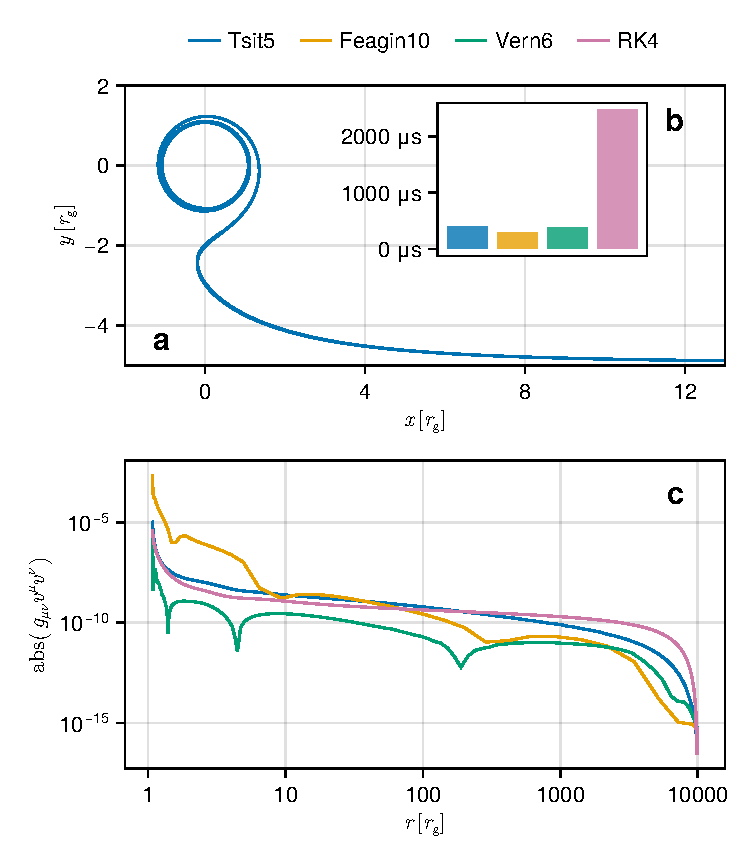
\includegraphics[width=0.95\linewidth]{figures/stability.conservation.pdf}
	\caption{\todo{caption + better choice of integrators to compare}}
	\label{fig:dot-stability}
\end{figure}

To test accuracy, we compare our numerical results with analytic values. The angular deflection is the difference in $x^\phi$ of a geodesic traveling from positive to negative infinity, that is
\begin{equation}
	\delta x^\phi :=
		x^\phi_{+\infty} - x^\phi_{-\infty} 
		- \pi,
\end{equation}
where the $-\pi$ is to account for radial change in the coordinate system between start and endpoint as the geodesic passes the origin \todo{is this right??}. Semi-analytic solutions for the deflection angle in the Kerr spacetime have been calculated for equatorial geodesics in \cite{iyer_lights_2009}, using elliptic integrals to find the coordinate differences. We follow their notation and denote the analytic deflection angle $\hat{\alpha}$, and present a compact summary of their calculations in Appendix \ref{appendix:deflection-angle}. 

Figure \ref{fig:deflection-angle} shows the deflection angle as a function of impact parameter $\alpha$ calculated using our code, along with the analytic deflection, and a measure of the error for different integration algorithms. Note the asymptotic behaviour of the error as $\lvert \alpha \rvert$ increases -- we account for this as related to the approximate observer at infinity in ray-tracing methods, catalyzed by the geometry of our observer introducing a small error at any finite $x^r$ when calculating the impact parameters relative to an $x^r = \infty$ observer. As can be expected, the error increases if $x^r_\text{start}$ is decreased.

\begin{figure}
	\centering
	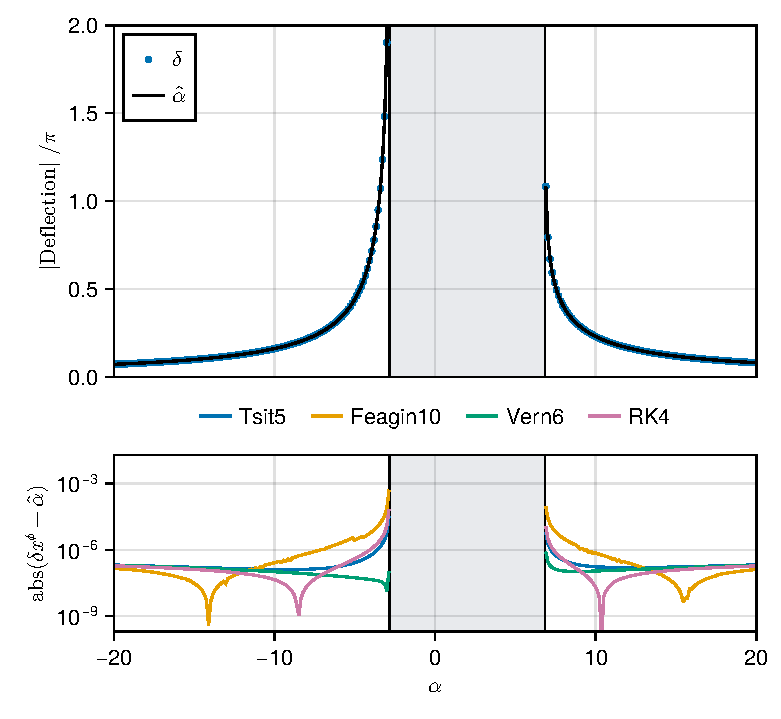
\includegraphics[width=0.94\linewidth]{figures/deflection.iyer-hansen.pdf}
	\caption{Deflection angle in the Kerr spacetime ($M = 1$, $a = 0.998$) for geodesics in the equatorial plane over a range of impact parameters $\alpha$. Upper panel: numerical deflection $\delta x^r$ calculated with  $x^r_\text{start} = 2 \times 10^8 \, \rg$, absolute and relative tolerances set to $10^{-14}$, and effective infinity $4 \times 10^8\, \rg$, shown with the numerical solutions for $\hat{\alpha}$. Lower panel: the absolute relative error between the numeric and analytic deflection angles for different integration algorithms.}
	\label{fig:deflection-angle}
\end{figure}


\todo{Energy conservation, deflection problem, shadow, tests for naked-singularities}


\subsection{Emissivity curves}

We calculate a number of emissivity profiles that have been published in the literature as a test of the numerical methods in Section \ref{sec:emissivity-profiles}. In Figure \ref{fig:emissivity-profiles} are shown the emissivity profiles for the lamp post corona at different heights, including the time difference due to the Shapiro delay. Our results are consistent with other authors \citep{wilkins_understanding_2012,dauser_irradiation_2013}.

\begin{figure}
	\centering
	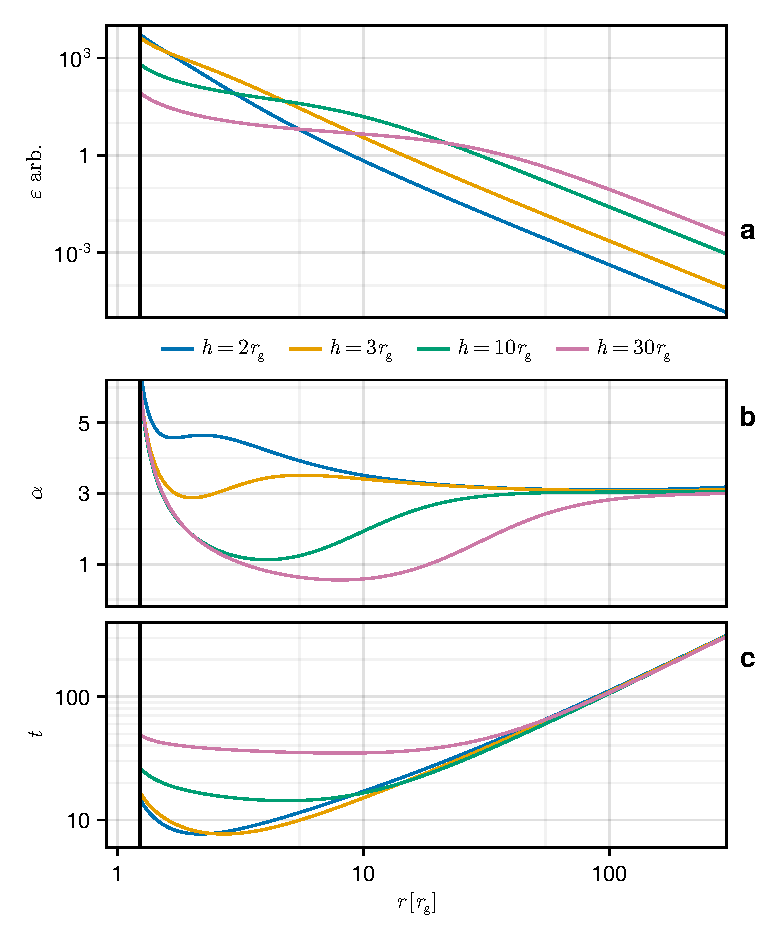
\includegraphics[width=0.99\linewidth]{figures/emissivity.point-source.pdf}
	\caption{\todo{caption}}
	\label{fig:emissivity-profiles}
\end{figure}

\todo{Wilkins and Fabian with lamp post and moving corona, gonzalez 2017}

\subsection{Line profiles}

Transfer functions are integrated as described in Section \ref{sec:transfer-function-integration}, neglecting the timing components. Figure \ref{fig:relline-comparison} compares the line profiles computed using the transfer functions of \Gradus and the \relline model of \cite{dauser_broad_2010}\footnote{We compare against the \relline model distributed in the Relxill package \url{http://www.sternwarte.uni-erlangen.de/~dauser/research/relxill/}, which is the latest version at time of publication (v2.3 with table v0.5a).}. We see good agreement to within $\sim 1\%$ accuracy, with all features collocated.

\begin{figure}
	\centering
	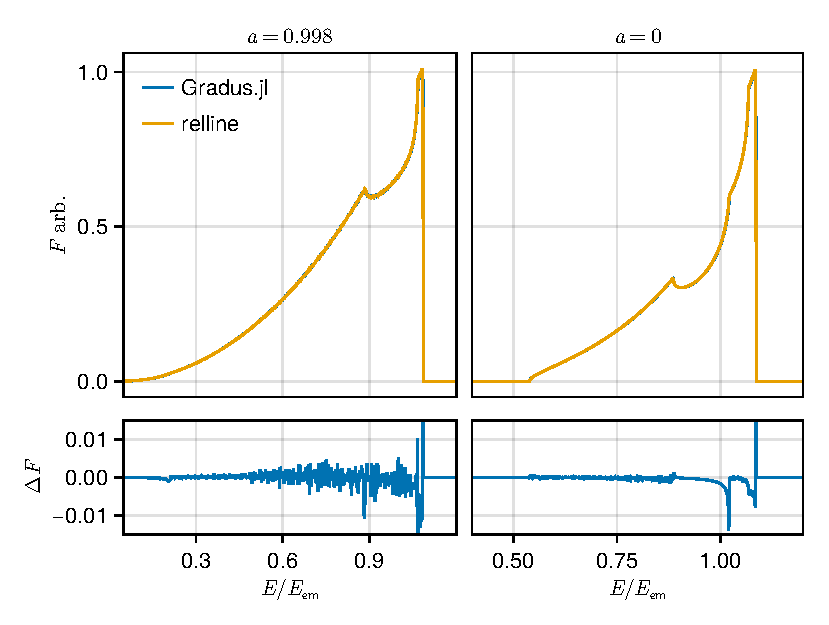
\includegraphics[width=0.99\linewidth]{figures/lineprofiles.comparison.pdf}
	\caption{Comparison of line profiles calculated by integrating transfer functions with emissivity $I_\text{em} = \varepsilon(r_\text{em}) = r_\text{em}^{-3}$ using \Gradus and \relline. The transfer functions are calculated for an observer at $r_\text{obs} = 1000\rg$ and $\theta_\text{obs} = 40^\circ$, and integrated between $r_\text{in} = r_\text{ISCO}$ and $r_\text{out} = 50 \rg$. Left panel is the the maximally spinning Kerr spacetime, whereas the right panel is the Schwarzschild spacetime.}
	\label{fig:relline-comparison}
\end{figure}

Our code permits a consistency check by binning geodesics on the image plane, with the appropriate weighting. This method may also be used to compute line profiles for accretion geometry that does not lend itself to the transfer function parameterization. In Figure \ref{fig:line-profile-ssd}, we compute a number of line profiles for the SSD, using both the binning and transfer integration approach. \todo{finish this section}

\begin{figure}
	\centering
	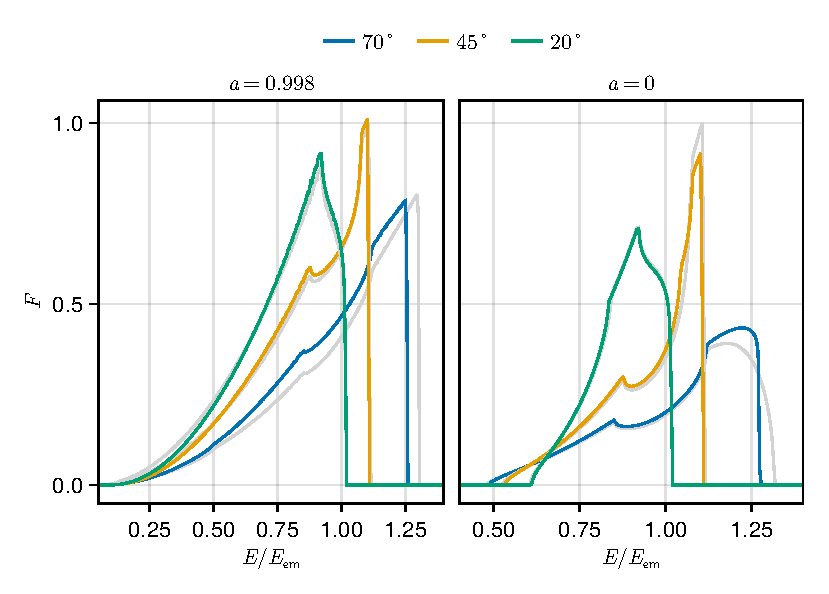
\includegraphics[width=0.99\linewidth]{figures/lineprofiles.ssd.pdf}
	\caption{Line profiles for the SSD with $\dot{M} / \dot{M}_\text{Edd} = 0.3$ for different observer inclinations $\theta_\text{obs}$ and emissivity $I_\text{em} = \varepsilon(r_\text{em}) = r_\text{em}^{-3}$. The transfer functions are calculated as in Figure \ref{fig:relline-comparison}, and integrated over the same limits. The light-grey lines correspond to the geometric thin disc ($\dot{M} / \dot{M}_\text{Edd} = 0$), and differ only for steep inclinations due to obscuration of inner $r_\text{em}$. Left panel is the the maximally spinning Kerr spacetime, whereas the right panel is the Schwarzschild spacetime.}
	\label{fig:line-profile-ssd}
\end{figure}


\subsection{Reverberation lags}
\label{sec:lag-transfer-functions}

\citep{reynolds_x-ray_1999,wilkins_origin_2013,cackett_modelling_2014}

\todo{Ingram's code? Jiachen's code}

\begin{figure}
	\centering
	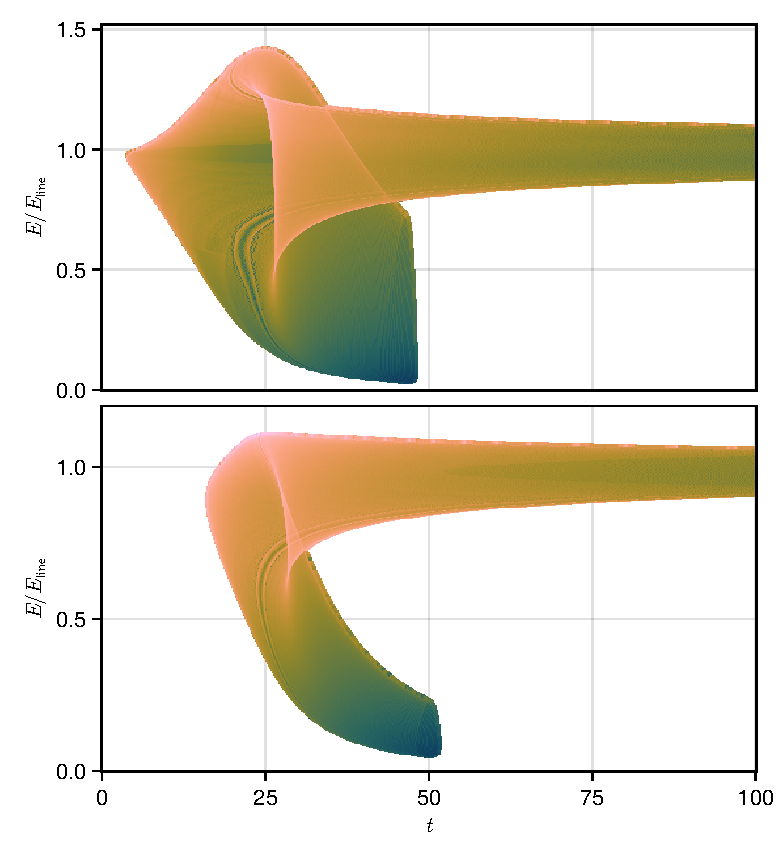
\includegraphics[width=0.97\linewidth]{figures/transfer-functions.2d.pdf}
	\caption{\todo{caption + slit is the gap between upper and lower branch contributions:: idea, interpolate when in h or 1-h}}
	\label{fig:lag-frequency-transfer-functions}
\end{figure}

\subsubsection{Lag-frequency spectra}

Summing the two dimensional transfer functions over the energy axis for a given energy range yields an impulse response $\psi(t)$, describing the time evolution of the observed flux. This impulse response depends on the properties of the illuminating corona, accretion disc, spacetime, and inclination of the observer. Examples for different lamp post heights over the full energy range are shown in the top panel of Figure \ref{fig:reverberation-thin}.

Following \cite{cackett_modelling_2014}, we define the \textit{response fraction} $R$ as the ratio of reflected to continuum flux. The impulse response in the Fourier domain is then the rescaled Fourier transform
\begin{equation}
	\mathscr{F}_\psi(f) := R \int_{0}^\infty \psi(t) \e^{-2\pi i f t} \d t.
\end{equation}
The phase difference between the reflected and continuum flux is 
\begin{equation}
	\phi(f) = \tan^{-1} \left( 
		\frac{\Im{\mathscr{F}_\psi}}{1 + \Re{\mathscr{F}_\psi}} 
	\right),
\end{equation}
where $\Im{\mathscr{F}_\psi}$ and $\Re{\mathscr{F}_\psi}$ are the imaginary and real components of $\mathscr{F}_\psi$ respectively. The imaginary component represents the lag contribution to the phase difference. Since the driving signal is present in both bands, it adds no lag contribution, but serves to dilute the phase difference and therefore the real component of the signal through the $+1$ in the denominator \citep{cackett_modelling_2014}. \todo{expand on this}

The time lag is defined as 
\begin{equation}
	\tau(f) := \frac{\phi}{2 \pi f},
\end{equation}
and relates the observed time lag to the Fourier frequency of the driving signal (lower panel of Figure \ref{fig:reverberation-thin}).

\begin{figure}
	\centering
	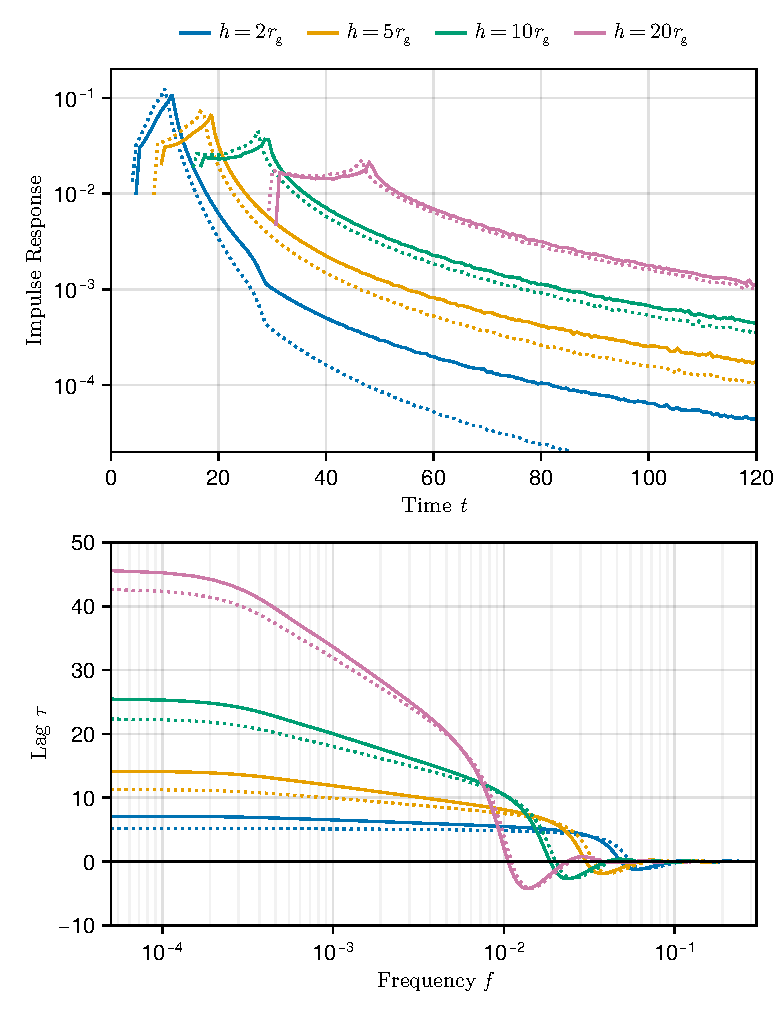
\includegraphics[width=0.98\linewidth]{figures/reverberation.thin-disc.pdf}
	\caption{\todo{TODO + move legend}}
	\label{fig:reverberation-thin}
\end{figure}

We note a slight disagreement with \cite{cackett_modelling_2014} in the $h = 10$ and $h=20$ case, due to a weak-field approximation after $100\, \rg$, which the authors employ for performance. At $\theta_\text{obs} = 45^\circ$ inclination, the time difference due to the weak-field approximation between the reflected and continuum band increases with $h$, resulting in their continuum component arriving \textit{early}. This results in a shift of the impulse response towards later $t$, and therefore a greater low frequency lag and a shift of the peak of the negative lag to lower $f$.
\todo{maybe put this in an appendix and explain better with figures??}

\subsubsection{Lag-energy spectra}

\begin{figure}
	\centering
	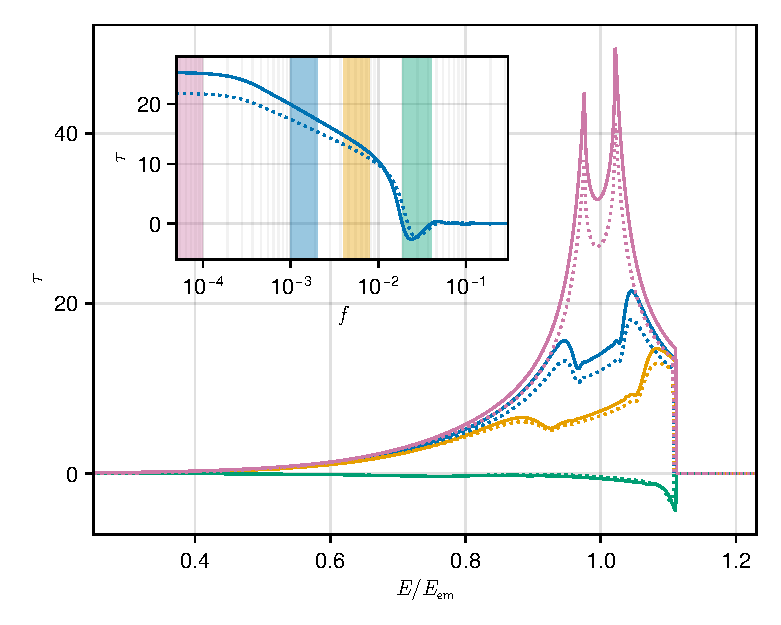
\includegraphics[width=0.98\linewidth]{figures/reverberation.lag-energy.pdf}
	\caption{\todo{TODO + move legend}}
	\label{fig:lag-energy}
\end{figure}


\subsection{Analytic radiative transfer model}

\cite{gold_verification_2020} specify an analytic model for testing radiative transfer codes (their Section 3.2, with results shown in their Figure 2 and 3). We have implemented their model and traced the radiative transfer problems with \Gradus, shown in Figure \ref{fig:gold-test-problems}. We find good agreement with the published results for all test problems.

\begin{figure*}
	\centering
	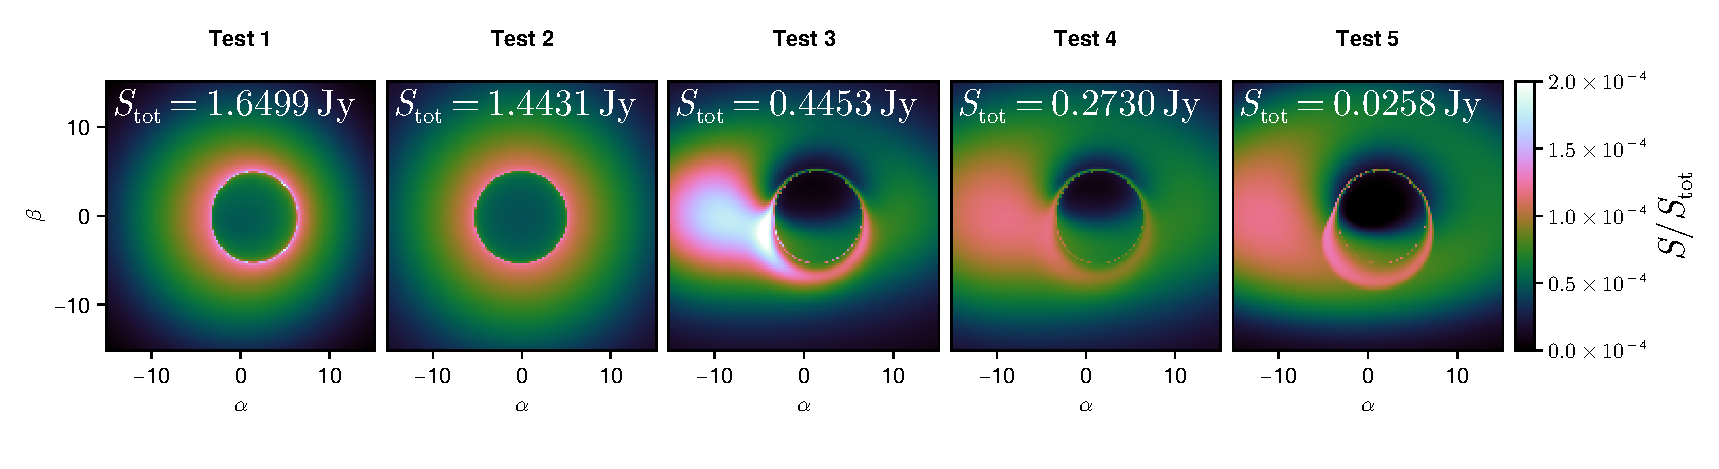
\includegraphics[width=0.99\linewidth]{figures/radiative-transfer.gold.pdf}
	\caption{Intensity images calculated with \Gradus of the radiative transfer analytic test models specified in \citet{gold_verification_2020} with resolution $128 \times 128$ pixels, and impact parameters ranging between $-15\, \rg$ and $15\, \rg$, and observer position $r_\text{obs} = 1000\, \rg$ and inclination $\theta_\text{obs} = 60^\circ$. The test cases correspond to the test parameters in their Table 1. The colouring is the intensity for the geodesic corresponding to that pixel normalized over the total intensity .}
	\label{fig:gold-test-problems}
\end{figure*}

\subsection{Other spacetimes}

\todo{Bambi's various metrics and relline, self consistency between methods}
\todo{iron line profiles for Johannsen Psaltis}
\todo{geodesic motion of kerr newman}

\section{Applications}

\todo{working on spectral and timing models (Baker et al. in prep) for use in XSPEC and beyond}

\todo{working on propagating gradient information from models into spectral fitting pipelines}

\todo{including radiative transfer information in the transfer functions}

We are working on a optimized thick disc spectral and reverberation model for use in spectral fitting programs based on our thick disc transfer functions and time-dependant transfer function integration. 

\section{Conclusions}

We encourage the community to contact us with interesting problems that may be tackled using \Gradus as we are happy to assist with new applications of the code.

\todo{problems with the code are being patched, see github issues}

% Note future work, e.g., with regard to fitting, and using the code in other papers

\section*{Acknowledgements}
This work is supported by the UKRI AIMLAC CDT funded by grant EP/S023992/1.

We thank Jiachen Jiang, Cosimo Bambi and Askar Abdikamalov for sharing their software for comparisons. FB thanks Rosie for her expert debugging assistance, and Shaun for invaluable software discussions. All figures created using Makie.jl \citep{DanischKrumbiegel2021}, using the color scheme of \cite{wong_points_2011}.

%%%%%%%%%%%%%%%%%%%%%%%%%%%%%%%%%%%%%%%%%%%%%%%%%%
\section*{Data Availability}

No new data or analyses have been created for this work. The code to reproduce this paper and all figures therein is freely available under MIT license:
\url{https://github.com/fjebaker/gradus-paper}


% The inclusion of a Data Availability Statement is a requirement for articles published in MNRAS. Data Availability Statements provide a standardised format for readers to understand the availability of data underlying the research results described in the article. The statement may refer to original data generated in the course of the study or to third-party data analysed in the article. The statement should describe and provide means of access, where possible, by linking to the data or providing the required accession numbers for the relevant databases or DOIs.

%%%%%%%%%%%%%%%%%%%% REFERENCES %%%%%%%%%%%%%%%%%%

% The best way to enter references is to use BibTeX:

\bibliographystyle{mnras}
\bibliography{citations} % if your bibtex file is called example.bib


%%%%%%%%%%%%%%%%%%%%%%%%%%%%%%%%%%%%%%%%%%%%%%%%%%

%%%%%%%%%%%%%%%%% APPENDICES %%%%%%%%%%%%%%%%%%%%%

\appendix

\section{orthonormalization with Gram-Schmidt}
\label{appendix:gram-schmidt}

The theorem of Gram-Schmidt states that it is always possible to construct a set of orthonormal vectors in any inner-product space $\mathbb{R}^n$, and uses a projection-subtraction procedure as a proof \citep{schmidt_uber_1989}. Starting with $n$ linearly independent vectors $\vector{v}_n$, and denoting the projection of a vector $\vector{u}$ along the direction of $\vector{v}$ as
\begin{equation}
\mathrm{P}_{\vector{v}}\left(\vector{u}\right) := \frac{\vector{v} \cdot \vector{u}}{\vector{u} \cdot \vector{u}}\ \vector{u} = \frac{g_{\mu\nu} v^\mu u^\nu}{g_{\sigma\rho} u^\sigma u^\rho} \vector{u},
\end{equation}
allows expressing the Gram-Schmidt procedure as
\begin{align}
    \vector{k}_1 &= \vector{v}_1, \nonumber \\
    \vector{k}_2 &= \vector{v}_2 - \mathrm{P}_{\vector{k}_1}\left(\vector{v}_2 \right), \nonumber \\
    &\vdots \nonumber \\
    \vector{k}_n &= \vector{v}_n - \sum_{i = 1}^{n-1} \mathrm{P}_{\vector{k}_i} \left(\vector{v}_n \right).
\end{align}
Constructing meaningful orthonormal frames requires appropriate choice of the initial linearly independent vectors $\vector{v}$, in order to associate global directions with the tetrad. The locally non-rotating frame (LNRF), with angular velocity $\omega = -g_{t\phi} / g_{\phi\phi}$, has tangential frame velocity $v^\mu = A (1, 0, 0, \omega)$ where $A$ is some normalization. To construct the LNRF, a choice of initial vectors may therefore be
\begin{align}
    \vector{v}_1 &= \left(1, 0, 0, \omega \right) \mapsto \dtensor{\e}{(t)}{\mu}, \nonumber \\
    \vector{v}_2 &= \left(1, 0, 0, 1\right) \mapsto \dtensor{\e}{(\phi)}{\mu}, \nonumber \\
    \vector{v}_3 &= \left(1, 1, 0, 1\right) \mapsto \dtensor{\e}{(r)}{\mu}, \nonumber \\
    \vector{v}_4 &= \left(1, 1, 1, 1\right) \mapsto \dtensor{\e}{(\theta)}{\mu},
\end{align}
where we have denoted the corresponding tetrad vector generated by the orthonormalization procedure after the arrow.

Other sensible frames require different initial vectors, and care must be taken in implementing a method that correctly reorders the resulting tetrad vectors: for example, the zero angular momentum (ZAMO) frame for an on-axis coronal source with velocity $\dot{x}^\mu = (1, \d r / \d t, 0, 0)$ requires
\begin{align}
    \vector{v}_1 &= \left(1, \d r / \d t, 0, 0 \right) \mapsto \dtensor{\e}{(t)}{\mu}, \nonumber \\
    \vector{v}_2 &= \left(1, 1, 0, 0\right) \mapsto \dtensor{\e}{(r)}{\mu}, \nonumber \\
    \vector{v}_3 &= \left(1, 1, 1, 0\right) \mapsto \dtensor{\e}{(\theta)}{\mu}, \nonumber \\
    \vector{v}_4 &= \left(1, 1, 1, 1\right) \mapsto \dtensor{\e}{(\phi)}{\mu}.
\end{align}

Our implementation of the Gram-Schmidt procedure is accurate up to machine-level with the analytic tetrads for the LNRF in \cite{bardeen_rotating_1972}, their Equation (3.2), and for the moving source ZAMO frame in \cite{gonzalez_probing_2017}, their Equation (10).

\section{Keplerian orbits of static, axis-symmetric spacetimes with accelerated geodesics}
\label{appendix:circular-orbits}
\section{Semi-analytic deflection angle for static, axis-symmetric spacetimes}
\label{appendix:deflection-angle}



% \section{Some extra material}

%%%%%%%%%%%%%%%%%%%%%%%%%%%%%%%%%%%%%%%%%%%%%%%%%%


% Don't change these lines
\bsp	% typesetting comment
\label{lastpage}
\end{document}

% End of mnras_template.tex
